\documentclass[12pt]{article}
\usepackage[utf8]{inputenc}
\usepackage{amssymb,latexsym,graphicx}
\usepackage{enumitem}
\usepackage{amsmath,amscd,amsthm}
\usepackage{mathrsfs}
\usepackage{amsrefs}
\usepackage{graphicx}
\usepackage{breqn}
\usepackage{tikz}
\usepackage{environ}
\usepackage{pgfplots}
\usepackage{gensymb}
\usepackage{math tools}
\usepackage[letterpaper, margin=1 in]{geometry}
\usepackage{relsize}
\usepackage{hyperref}
\hypersetup{
    colorlinks=true,
    linkcolor=black,
    filecolor=black,      
    urlcolor=black,
    citecolor=black,
}
%\pgfplotsset{compat=1.14}

\usepackage{chngcntr}
%%%%%%%%%%%%%%
\setlength{\parskip}{8pt}
\setlength\parindent{24pt}
\pagenumbering{arabic}

%%%%%%%%%%%%% NICE COLOURS (imported manually from http://latexcolor.com/)
\definecolor{forest}{rgb}{0.13, 0.55, 0.13}
\definecolor{brandeisblue}{rgb}{0.0, 0.44, 1.0}	
\definecolor{cadmiumorange}{rgb}{0.93, 0.53, 0.18}


%%%%%%%%%%%%% MAIN TEXT
\title{Guidelines and Tips for Making Figures}
\author{Adam Morgan
\\
adam.morgan@mail.utoronto.ca
}
\date{\today}

\begin{document}
\maketitle

\section{Introduction}
\noindent 
%In Homework 4, you are asked to produce many different plots. 
The effective presentation of figures is a critical skill for the modern scientist, one that requires a huge amount of practice to perfect. In this document included I've some concrete suggestions of software packages you may find useful to help make your figures. More importantly,  I've outlined general rules to follow when preparing images to supplement mathematical/scientific discussions. I conclude by drawing a few example pictures to bring the guidelines to life. 
%\par \noindent 
%\textit{Disclaimer}: You are not forced to make pictures on a computer for Homework 4. However, in my experience plots made with a computer are much cleaner, clearer, and overall more effective than those drawn by hand. So, chances are a computer-drawn plot will score higher on the assignment than a hand-drawn one. The guidelines below will be useful to you whether or not you choose to use a computer to make your figures. 

\section{Suggestions of Free Plot-Making Software}
\noindent
These packages are quite popular and well-documented, so with some Googling you can quickly figure out how to do pretty much anything you want with either of them (for this reason, I won't give you a comprehensive tutorial on these packages here). 
\par \noindent 
\textit{Disclaimer}: The following packages represent my own personal preferences and do not constitute an exhaustive list of high-quality, free plotting software. 
\begin{itemize}
\item TikZ (including pgfplots): a nice way to produce figures from TeX files. This is what I used to make the figures in this document. See
$$ \href{https://www.overleaf.com/learn/latex/Pgfplots_package}{\texttt{overleaf.com/learn/latex/Pgfplots_package}}
$$ 
to learn the basics. Pretty easy to use but can run slowly if you're making lots of pictures so be warned. Has the advantage of coming with most installations of \LaTeX. 
\item Matplotlib (see \href{https://matplotlib.org/}{\texttt{matplotlib.org}}): a Python library that is very versatile, very elegant, and very easy to use. Also an industrial favourite. I think Matplotlib comes with NumPy, so if you have a version of Python from the last few years you probably have it on your computer already. 
\item MATLAB (see \href{https://www.mathworks.com/}{\texttt{mathworks.com}}): a very user-friendly pay-to-use software for all types of scientific computing. MATLAB's plotting package can do essentially anything Matplotlib does. If you're a student, you can probably get MATLAB for free or at a big discount through your institution. There are also free MATLAB alternatives like Octave, but I haven't used these much and so can't vouch for them. 
\end{itemize}

\section{Guidelines for Making Figures}
\begin{itemize}
    \item \textbf{The Golden Rule}: When looking at one of your figures always ask yourself, ``would I understand and appreciate this picture if I saw it in a book or a research article?"... if your answer is ``no" then the figure is not finished. 
    \item Make sure every figure tells a story. Think of \emph{why} a piece of information must be described visually, and make sure your figure is focused on conveying that information.  
    \item Label axes clearly. 
    \item Label different curves on the same axes clearly. 
    \item Any points in the plane that are important to the story of the picture should also be labelled. 
    \item Include as many tick marks on your axes as necessary to communicate the big idea of your picture. Sometimes none at all is OK. 
    \item Make sure the font size on all your labels is appropriate. 
    \item Use concise captions. Don't be afraid to defer discussion to the body of the text. 
    \item A figure shouldn't be so densely packed that there's only a small amount of empty white space: such space gives our eyes a rest. Too much white space, however, has no use and can often distract the reader from the important point of an image. 
    \item If your picture includes a legend, make sure it does not cover any vital part of the image. 
    \item Even very good software like Matplotlib sometimes defaults to saving pictures with poor resolution. So, while you see a beautiful image when you run your code, it ends up looking blurry when you add it to a document! The fix for this is to manually change the resolution of the image, which is very easy. You want to Google something like ``how to change dpi in [insert software here]" (dpi stands for `dots per inch'). I find that a dpi of 600 is usually pretty OK. 
    \newpage
    \item \textbf{Choose colours carefully}.
    \begin{itemize}
    \item Many people cannot distinguish certain pairs of colours, and when designing a figure you should (to the best of your ability) make sure it is accessible to such readers. For a demonstration of the importance of colourblind-accessibility and several examples of colourblind-friendly palettes, see
    $$\href{https://davidmathlogic.com/colorblind}{\texttt{davidmathlogic.com/colorblind}}.$$
    \item Additionally, even those with full-colour vision may want to print off your figure in black-and-white (BW). So, the figure should still be understandable to these people too. 
         \item In general, I find the default colours in most software packages (including Tikz and Matplotlib) are not only non-accessible: they look terrible too. Fortunately, using alternatives is very easy. For pgfplots/TikZ, you can select from a huge list of colours available at \href{http://latexcolor.com/}{\texttt{latexcolor.com}}: just paste the colour definition into your TeX file and it's ready to be used. For Matplotlib (if you use a new-ish version), you can use any colour from the XKCD colour survey. See \href{https://xkcd.com/color/rgb/}{\texttt{xkcd.com/color/rgb}} for a list of these colours and their names. To use the XKCD colours in MATLAB, you'll need to download the package at $$ \hspace{-2cm}\href{https://www.mathworks.com/matlabcentral/fileexchange/46872-intuitive-rgb-color-values-from-xkcd}{\texttt{mathworks.com/matlabcentral/fileexchange/46872-intuitive-rgb-color-values-from-xkcd}}.$$  
         \item Try to stick with matte or pastel colours when possible. These are generally the most pleasing (or, if you're a pessimist, the least migraine-inducing) colours to look at. 
         \item When including different curves on the same axes, make them different colours and give them different styles (solid, dashed, dotted, etc.). 
         \item If you want to include a filled contour plot, don't use the ``jet" colourmap. In Matplotlib, some of the built-in colourmaps are better, but most of the time I stick to the cmocean colourmaps (see \href{https://matplotlib.org/cmocean}{\texttt{matplotlib.org/cmocean}}) which must be downloaded separately (if you use Python, \texttt{pip install cmocean}). 
        \end{itemize}
\end{itemize}

\section{Good and Bad Examples}
\noindent Let's apply the above guidelines to draw a nice, clear plot illustrating the behaviour of the heat kernel
$$
S(x,t) \doteq \frac{1}{2\sqrt{\pi \kappa t}}\exp\left(-\frac{x^2}{4\kappa t}\right)
$$
as time evolves. This plot is made using pgfplots. I will provide you with the raw TeX file for this document so you can see the code yourself (make sure you import TikZ and pgfplots in the preamble). 
\par Figure \ref{fig:heat_kernel_good} is drawn according to the guidelines above: labels are clear, the curves are distinguishable by both colour and style, the colours in the picture are muted and do not hurt the eyes (they are custom colours from \href{http://latexcolor.com/}{\texttt{latexcolor.com}}), and the picture is not too cramped (there is just enough white space). All of this makes it easy to see the mathematical idea being illustrated in the picture, namely that the heat kernel decays in amplitude and spreads out as time elapses; further, this spread becomes slower over time. 
\par However, seeing some examples of bad pictures may make the ideas stick in your head better. Figures \ref{fig:heat_kernel_bad1} and \ref{fig:heat_kernel_bad2} plot the exact same information as Figure \ref{fig:heat_kernel_good} (they even feature the same legend and labels). Both these new figures are much less effective than the original one: 
\begin{itemize}
    \item Figure \ref{fig:heat_kernel_bad1}: looking at this picture is painful! All three lines are solid so they couldn't be distinguished in a BW printed version, the colours are too bright and hurt the eyes (these are the default TikZ blue, yellow, green), and in places the green and yellow are difficult to distinguish even by a person like me with full-colour vision. 
    \item Figure \ref{fig:heat_kernel_bad2}: while this time the curves look good, the axes are all messed up: the $x$-axis is asymmetric for no good reason, and the $y$-axis goes up and down way too much. This figure is $75\%$ useless white space. The reader might be tricked into thinking there is some hidden information in the far regions of the image they need to focus on, otherwise why would the image's author format it so strangely? 
\end{itemize}
Hopefully, you have learned that a few easy choices can really make the difference in turning a horrible figure into a pleasant one. 
\begin{figure}
\centering
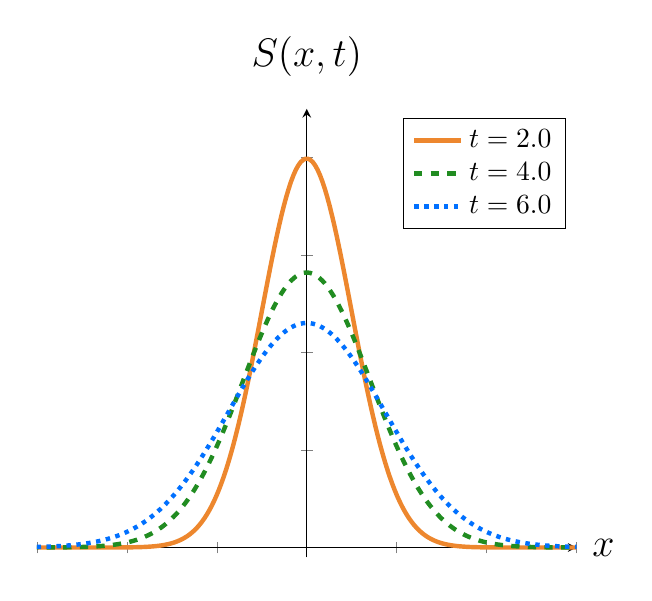
\begin{tikzpicture}[scale=1.0]
\begin{axis}[xmin=-6, xmax=6, ymin=-0.01, ymax=0.45, samples=300, no markers,
      axis x line = middle,
      axis y line = middle,
    ylabel=\Large{$S(x,t)$},
    xlabel=\Large{$x$},
    every axis x label/.style={
    at={(ticklabel* cs:1.05)},
},
every axis y label/.style={
    at={(ticklabel* cs:1.05)},
    anchor=south,
},
yticklabels={,,},
xticklabels={,,},
]
  
    \addplot[cadmiumorange, ultra thick, domain=-8:8]  {(1/sqrt(pi*2))*exp(-x*x/2)};
  \addlegendentry{$t=2.0$}
 
  
          \addplot[forest, ultra thick, domain=-8:8, dashed]  {(1/sqrt(pi*4))*exp(-x*x/4)};
  \addlegendentry{$t=4.0$}
  
    \addplot[brandeisblue, ultra thick, domain=-8:8, dotted]  {(1/sqrt(pi*6))*exp(-x*x/6)};
  \addlegendentry{$t=6.0$}
  
\end{axis}
\end{tikzpicture}
\caption{A nice plot illustrating the evolution of the heat kernel. Example of a good ``real" caption for this figure: Plot of the heat kernel $S(x,t)$ at various times $t$ for $\kappa=1/4$. As time elapses, the maximum over $x$ becomes smaller, and the width of the curves increases more slowly.} 
\label{fig:heat_kernel_good}
\end{figure}

\begin{figure}
\centering
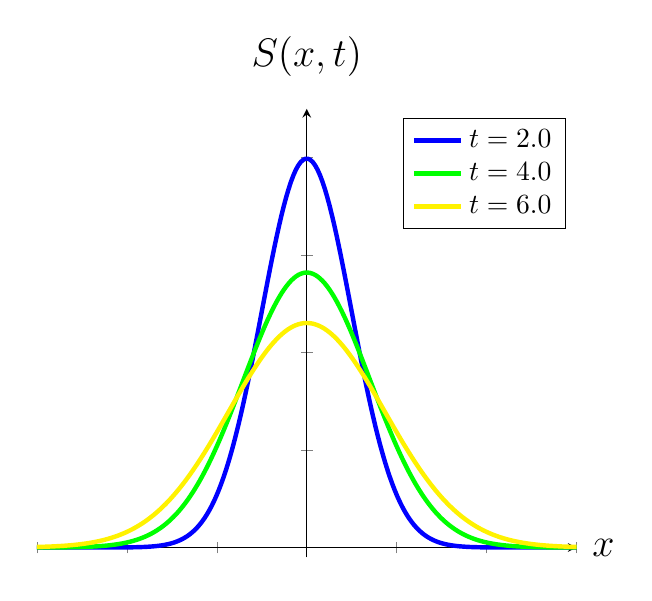
\begin{tikzpicture}[scale=1.0]
\begin{axis}[xmin=-6, xmax=6, ymin=-0.01, ymax=0.45, samples=300, no markers,
      axis x line = middle,
      axis y line = middle,
    ylabel=\Large{$S(x,t)$},
    xlabel=\Large{$x$},
    every axis x label/.style={
    at={(ticklabel* cs:1.05)},
},
every axis y label/.style={
    at={(ticklabel* cs:1.05)},
    anchor=south,
},
yticklabels={,,},
xticklabels={,,},
]
  
    \addplot[blue, ultra thick, domain=-8:8]  {(1/sqrt(pi*2))*exp(-x*x/2)};
  \addlegendentry{$t=2.0$}
 
  
          \addplot[green, ultra thick, domain=-8:8]  {(1/sqrt(pi*4))*exp(-x*x/4)};
  \addlegendentry{$t=4.0$}
  
    \addplot[yellow, ultra thick, domain=-8:8]  {(1/sqrt(pi*6))*exp(-x*x/6)};
  \addlegendentry{$t=6.0$}
  
\end{axis}
\end{tikzpicture}
\caption{A bad version of Figure \ref{fig:heat_kernel_good}. Do not make pictures like this!} 
\label{fig:heat_kernel_bad1}
\end{figure}

\begin{figure}
\centering
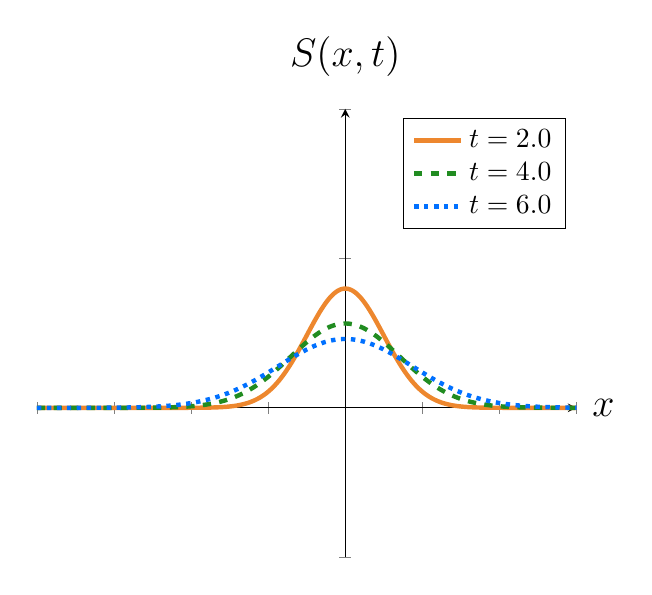
\begin{tikzpicture}[scale=1.0]
\begin{axis}[xmin=-8, xmax=6, ymin=-0.5, ymax=1., samples=300, no markers,
      axis x line = middle,
      axis y line = middle,
    ylabel=\Large{$S(x,t)$},
    xlabel=\Large{$x$},
    every axis x label/.style={
    at={(ticklabel* cs:1.05)},
},
every axis y label/.style={
    at={(ticklabel* cs:1.05)},
    anchor=south,
},
yticklabels={,,},
xticklabels={,,},
]
  
    \addplot[cadmiumorange, ultra thick, domain=-8:8]  {(1/sqrt(pi*2))*exp(-x*x/2)};
  \addlegendentry{$t=2.0$}
 
  
          \addplot[forest, ultra thick, domain=-8:8, dashed]  {(1/sqrt(pi*4))*exp(-x*x/4)};
  \addlegendentry{$t=4.0$}
  
    \addplot[brandeisblue, ultra thick, domain=-8:8, dotted]  {(1/sqrt(pi*6))*exp(-x*x/6)};
  \addlegendentry{$t=6.0$}
  
\end{axis}
\end{tikzpicture}
\caption{Another bad version of Figure \ref{fig:heat_kernel_good}. Do not make pictures like this!} 
\label{fig:heat_kernel_bad2}
\end{figure}



\end{document}
